% Theoretical background

\chapter{Theoretical background} \label{ch:theor_backgr}

This project is developed on top of another students final year project \cite{theseus:gere-zoltan} to automate the tasks that are required in the beginning of each course that uses their implementation.
Their solution provided the \gls{lora} end device, Chirpstack network server and LORIX One Gateway as starting tools.
The following section is a walk-through for the use of these elements without the implementation this project provides.

The end devices that the students use are added to an Application in Chirpstack server.
The server has clear \gls{ui} which is opened to the Applications page when the user logs in as seen in figure \ref{fig:chirpstack_application_list}.
From there the user can either choose an existing application or create new one.
Normally when a new course is organized the educator creates a new application for that class and all the related and used \gls{lora} end devices are added to that.

\begin{figure}[ht]
  \centering
  \AltText{Chirpstack network server's list of applications is shown}{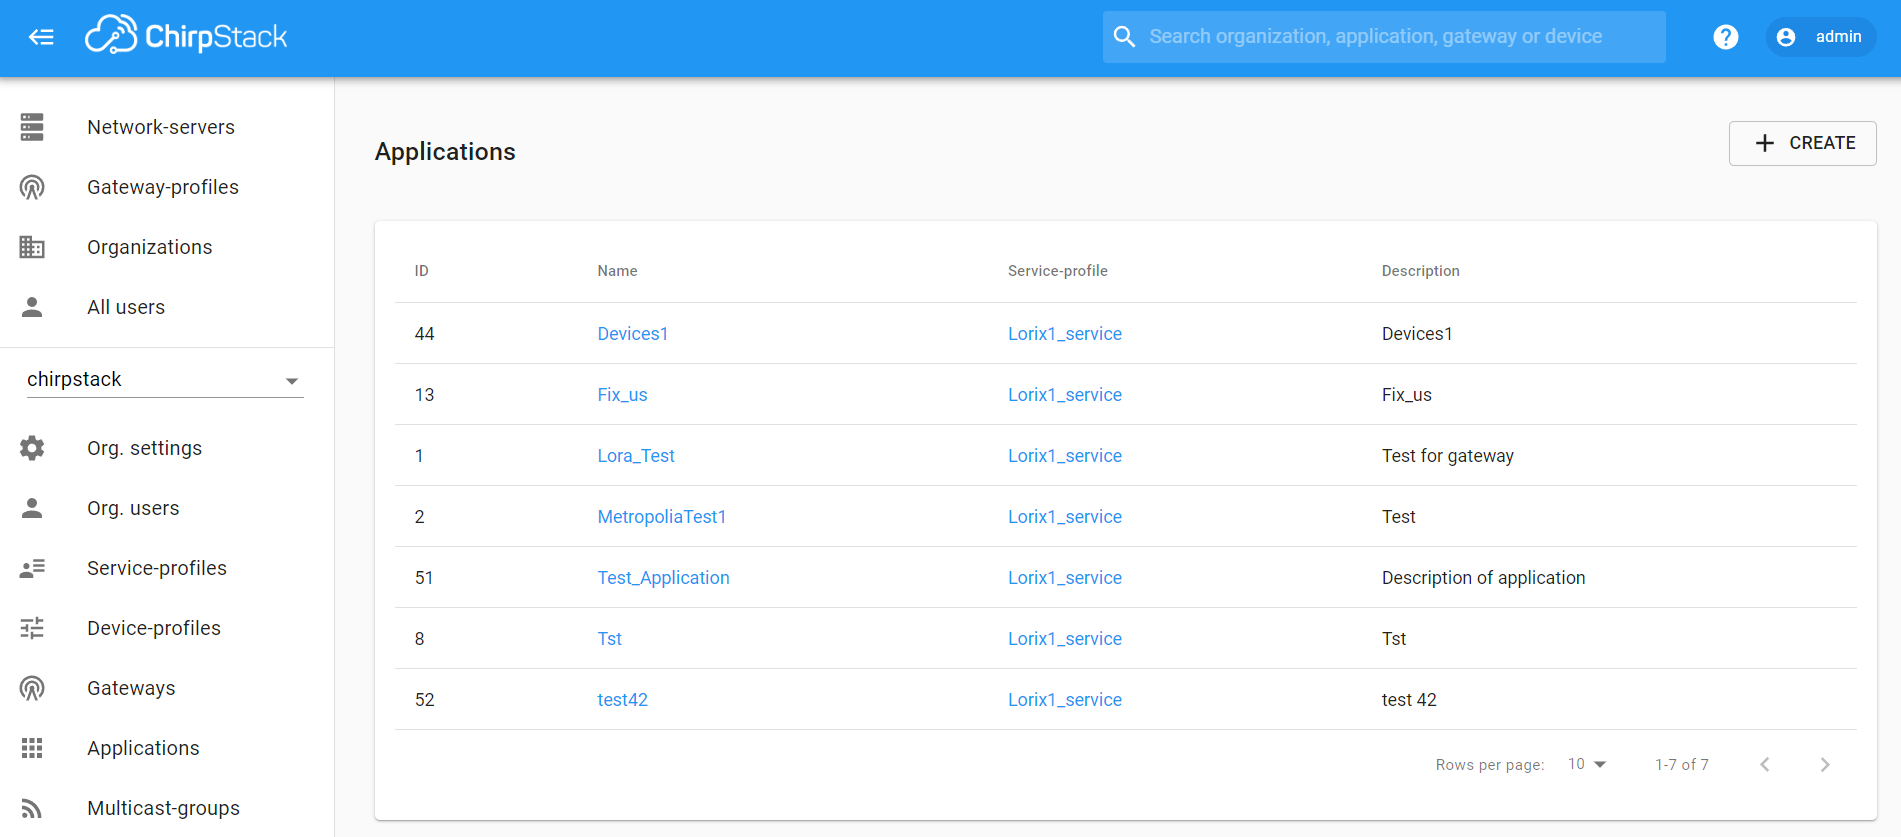
\includegraphics[width=\textwidth]{illustration/Chirpstack_application_list.png}}
  \caption{List of applications on a Chirpstack network server}
  \label{fig:chirpstack_application_list}
\end{figure}

In order to create a new application the user (educator) clicks the create button from the application layout and a new view opens with a from that has three mandatory fields to fill shown in figure \ref{fig:chirpstack_new_application}.
These fields are the application name, application description, and Service-profile of the application.
The first two are text input fields and the third one is a dropdown menu.
After filling up the required information that the use clicks the create application button and the application is generated.
The page then proceeds back to the list of application.

\begin{figure}[ht]
  \centering
  \AltText{Form to create a new application to Chirpstack server}{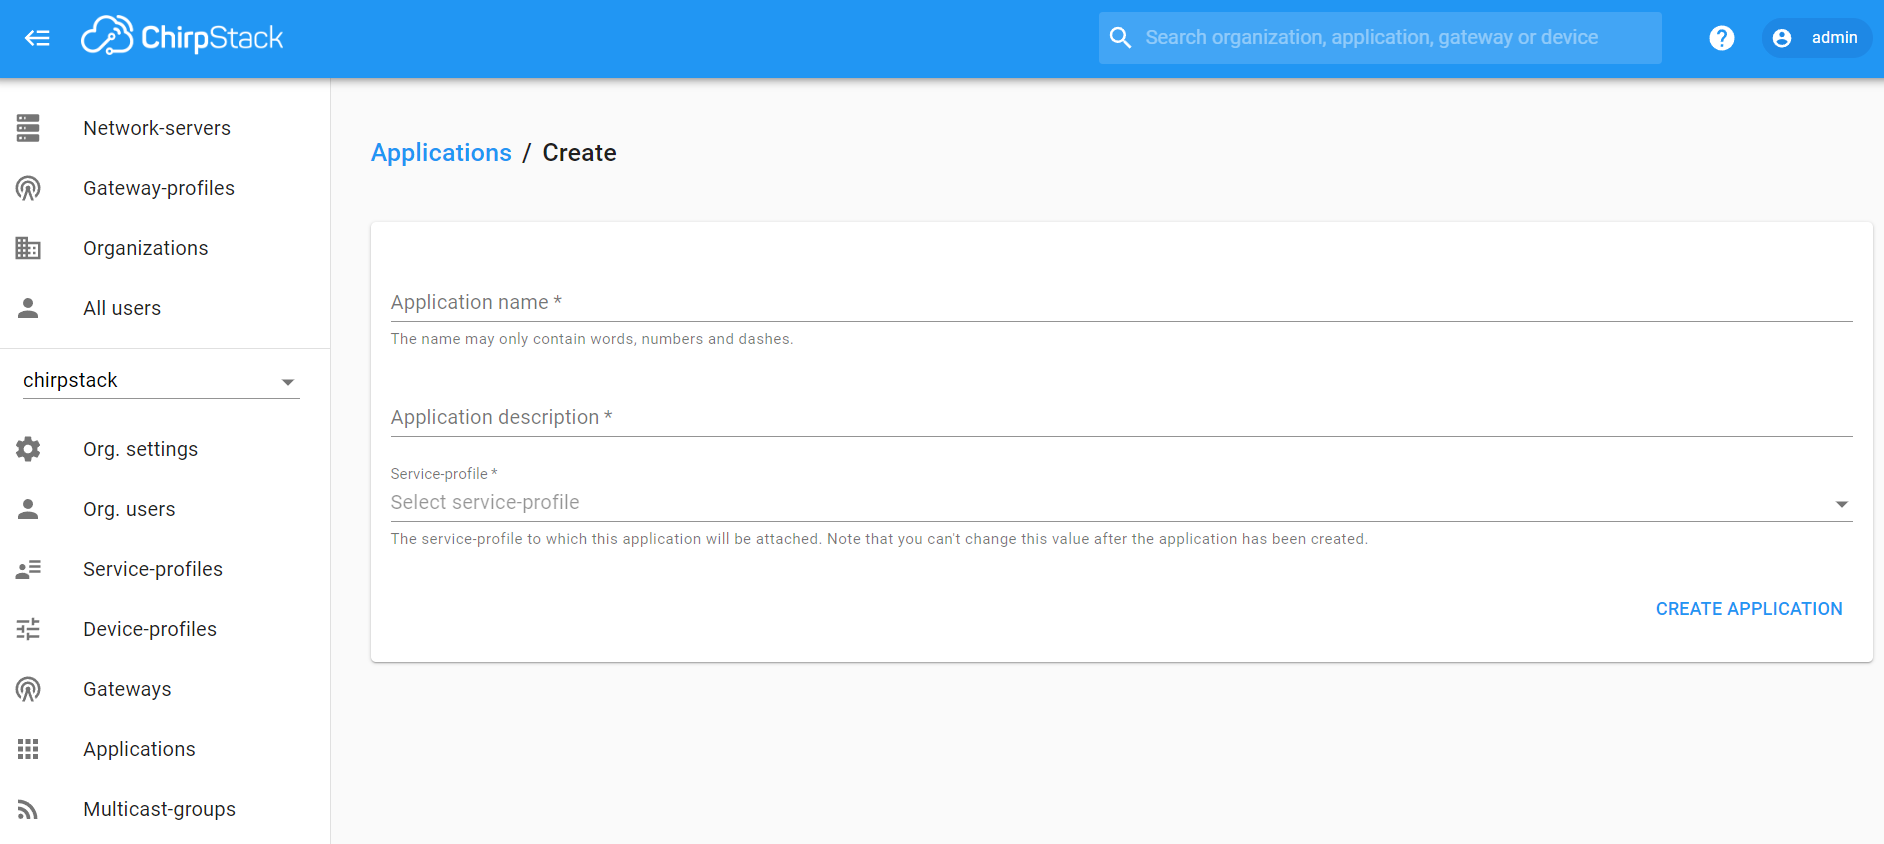
\includegraphics[width=\textwidth]{illustration/Chirpstack_new_application.png}}
  \caption{The new application creation form}
  \label{fig:chirpstack_new_application}
\end{figure}

When the desired application is opened a new layout with a list of current added devices for that application is shown.
When a new application is opened the device list is empty but visible.
That layout is opened to the Devices heading which is one of the four available ones that an application contains.
The other headings which can be selected are Application configuration, integrations and \gls{fuota}.
Application configuration contains the current information of the application name and description.
Those can be updated from there if needed.
Integrations shows a list of added integrations and new ones can be included from there with a list of available ones on a dropdown menu if create button is pressed there.
\gls{fuota} layout provides information about the Firmware Update Over the Air.
This feature is not used in the classes the school provides and therefor not included in the project. 

The device list shows each linked device provided with the information of when it is last seen, what are the device name and the device EUI, Link margin of the device and the latest information about the battery as seen in figure \ref{fig:chirpstack_application}.
For a user to add devices to the application certain information for that is required.

\begin{figure}[ht]
  \centering
  \AltText{Chirpstack network server's list of devices on application is shown}{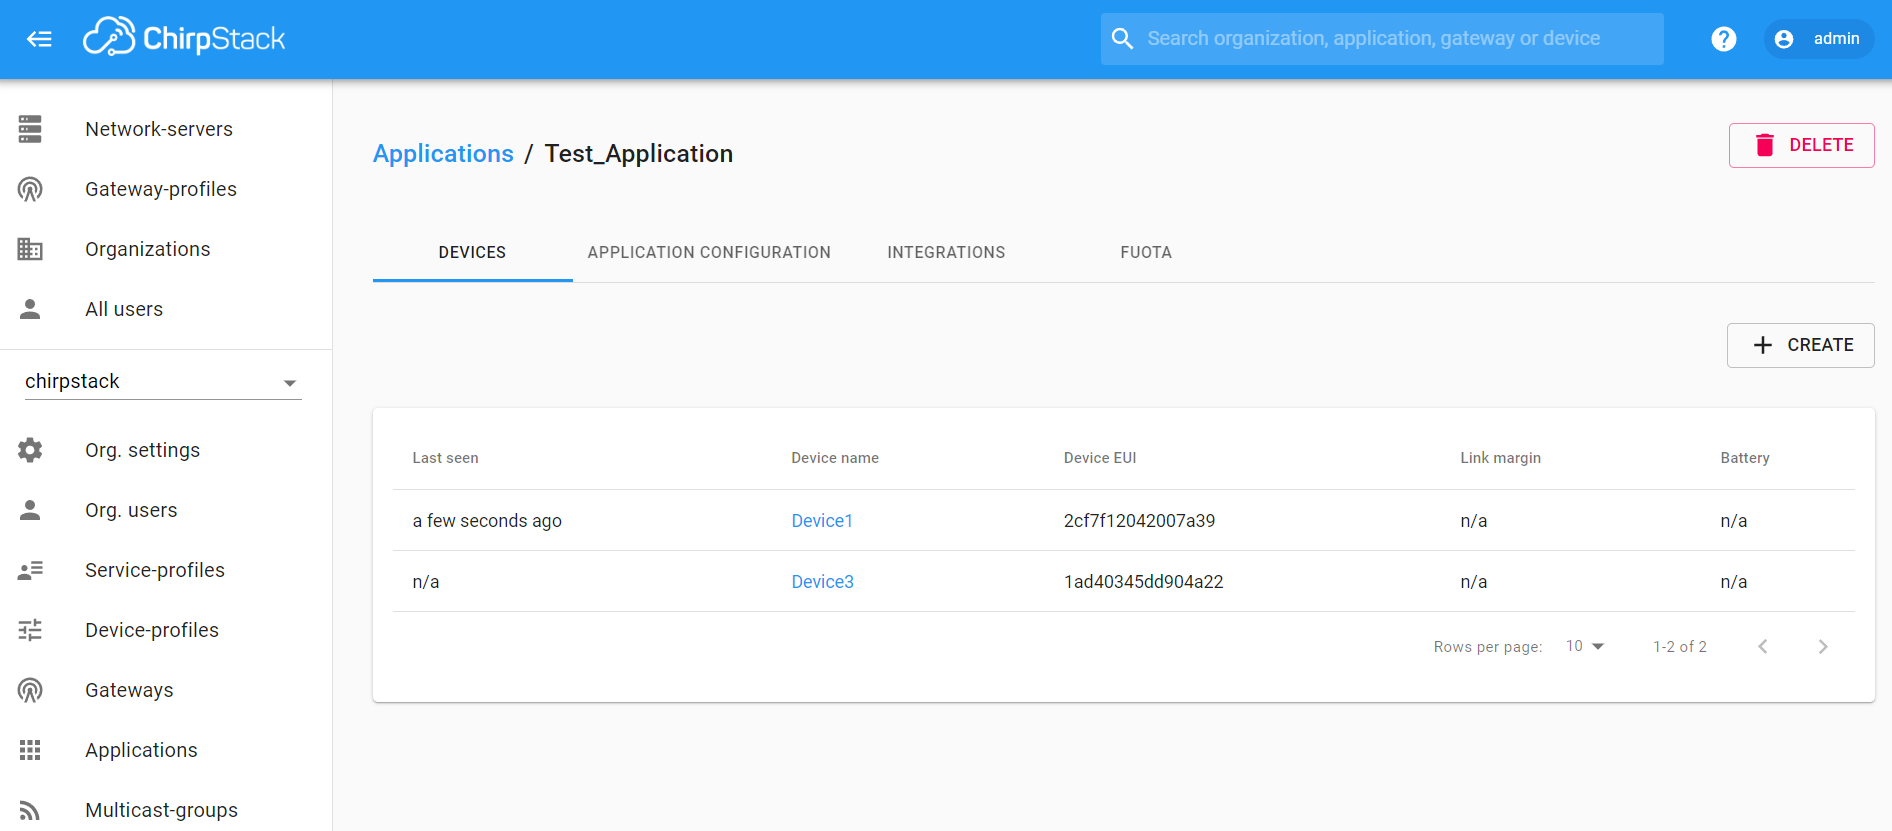
\includegraphics[width=\textwidth]{illustration/Chirpstack_application.png}}
  \caption{List of devices attached on application on a Chirpstack network server}
  \label{fig:chirpstack_application}
\end{figure}

When create button is pressed in the application layout the \gls{ui} opens a create form to connect the new device.
This form has three sections, general, variables, and tags as seen on figure \ref{fig:chirpstack_new_device}.
For this project only the general section needs to be focused on.
The General section has four mandatory fields.
In order to proceed to the next step device name, device description, device EUI and device-profile must be filled.
Device name and description are decided by the educator.
Device EUI can be found when the device is turned on and the Python script main.py is run.
Lastly the device-profile is selected from a dropdown menu.
The Chirpstack's layout also provides the possibility to generate a random ID for the device EUI, to toggle the byte order of it, and to check a box that disables the frame-counter validation.
These features are not used in the project.

\begin{figure}[ht]
  \centering
  \AltText{First layout form for adding a new device to Chirpstack server's application}{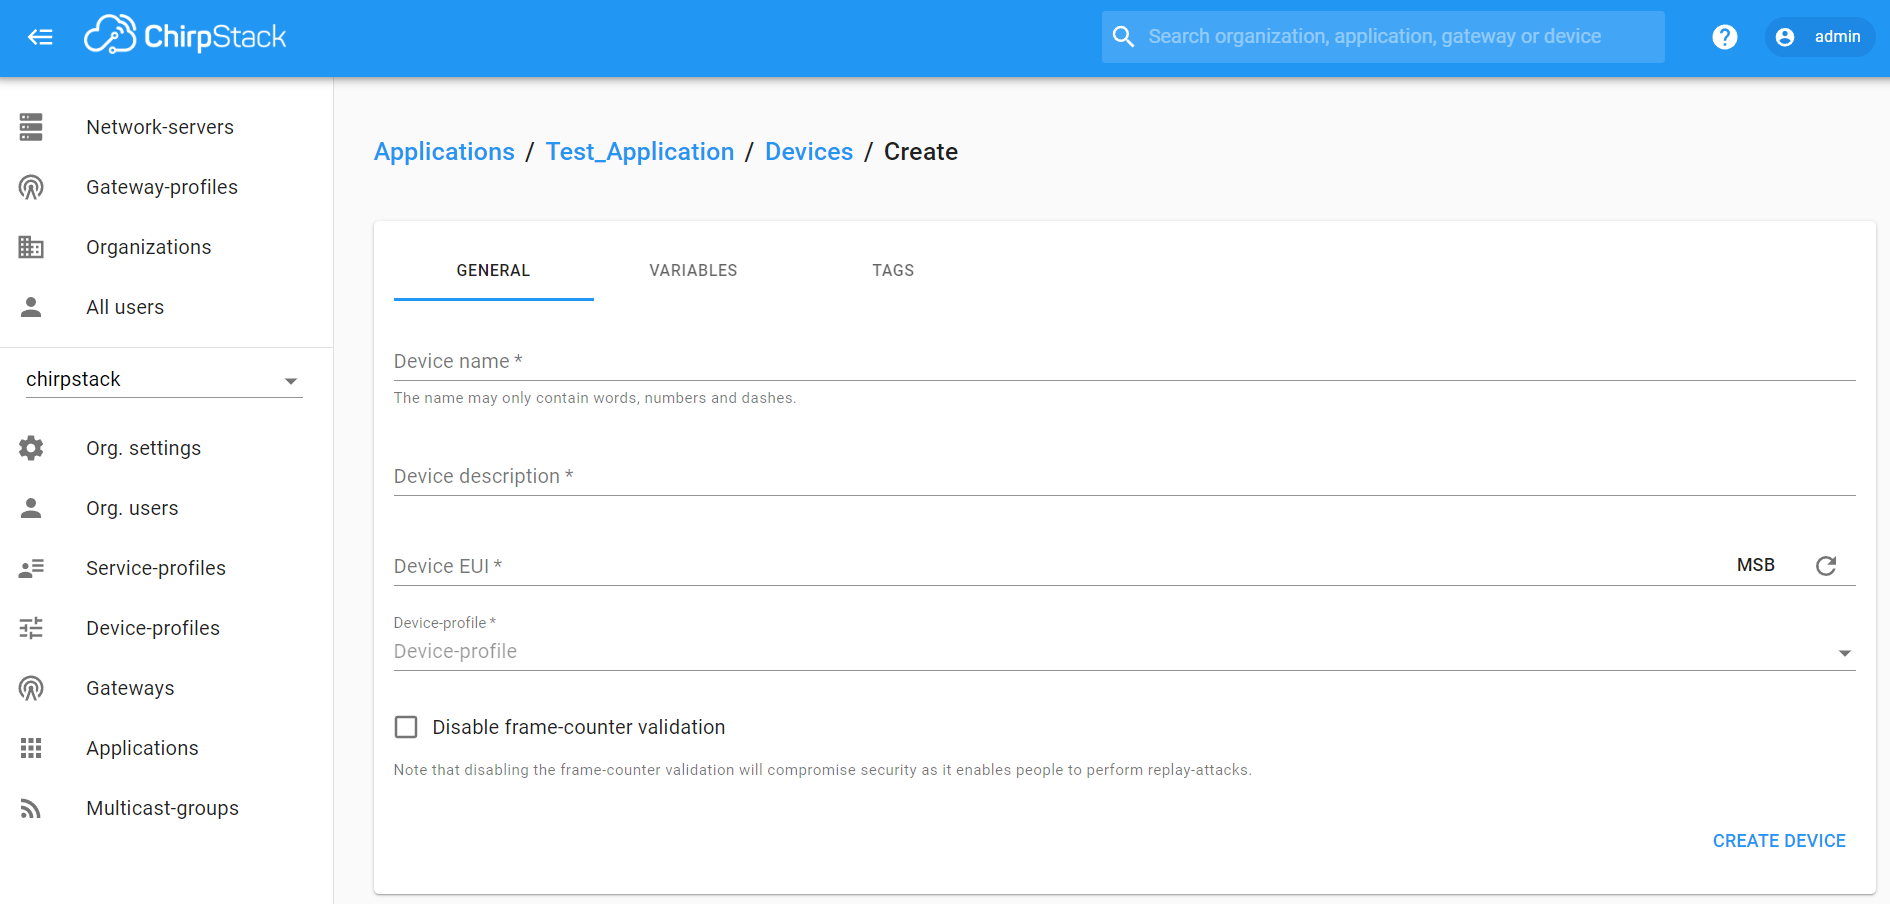
\includegraphics[width=\textwidth]{illustration/Chirpstack_new_device.png}}
  \caption{General information form for adding a new device to the application}
  \label{fig:chirpstack_new_device}
\end{figure}

After required information is given the user clicks Create Device button.
This process creates and adds the device to the application and the page uploads a layout of the device's Keys(\gls{otaa}) information as seen on figure \ref{fig:chirpstack_new_device_2}. 
The opened device has seven tab headers in total, that are details, the current Keys (\gls{otaa}), activation, device data, \gls{lorawan} frames, and firmware.
Next the information about the content of those tabs is explained.

Details layout has four text boxes called Details, Status, Enqueue downlink payload, and Downlink queue.
Details and Status boxes are visible all the time after a device is added to the application but theEnqueue downlink payload and Downlink queue only become visible after the device has been connected to the server for the first time.

Details shows the name and description of the opened device and a hyperlink to the Device-profile that has been selected for it.
The hyperlink leads to the general configuration page of that device-profile.
Status textbox has a Last seen at field that provides the information of the latest time that the device has been connected on the application.
Enqueue downlink payload provides possibility to transmit data to a queue from where it is sent to the \gls{lora} device. For this to happen, the user needs to give a port number and a Base64 encoded string or a JSON object and they can also tick a box  that the downlink is confirmed.
Downlink queue shows  a list of the downlinks that are on the queue while providing the main informations about them in four columns.
The downlink features are not used in the courses currently.

Configuration layout is the same one as when the user had clicked the create button on the application's devices header \ref{fig:chirpstack_new_device}.
From there the user can modify the general details of the device if wanted.
If this is done the new information is saved by pressing the update device button.
When the details are updated the page layout goes to Details tab where the modified data can be seen.

Keys (\gls{otaa}) layout is the one that was opened when the first step of the creation was done.
This text box has two fields, Application key and Gen application key.
Application key is a mandatory field and Gen Application key is optional.
The Application key is got when the Python main.py file from the device is ran.
Gen Application key is only needed when the device implements remote multicast setup specification or \gls{fuota}.
As neither of those features are not used in the implementation that field is left empty.

Activation layout provides a textbox with five fields when the device has been connected to the server / activated.
First field shows the Device address which is specified when the device has joined a network.
Network session key and Application session key are masked.
The concealed information can be seen by pressing the key icons next to the next fields.
The other two fields show the Uplink frame-counter and Downlink frame-counter information.

Device data layout sends uplink information from the device when it is connected in 5 second intervals.
If it is not activated the box instead shows a text "This device has not been (yet) activated".


\begin{figure}[ht]
  \centering
  \AltText{Second layout form for adding a new device to Chirpstack server's application}{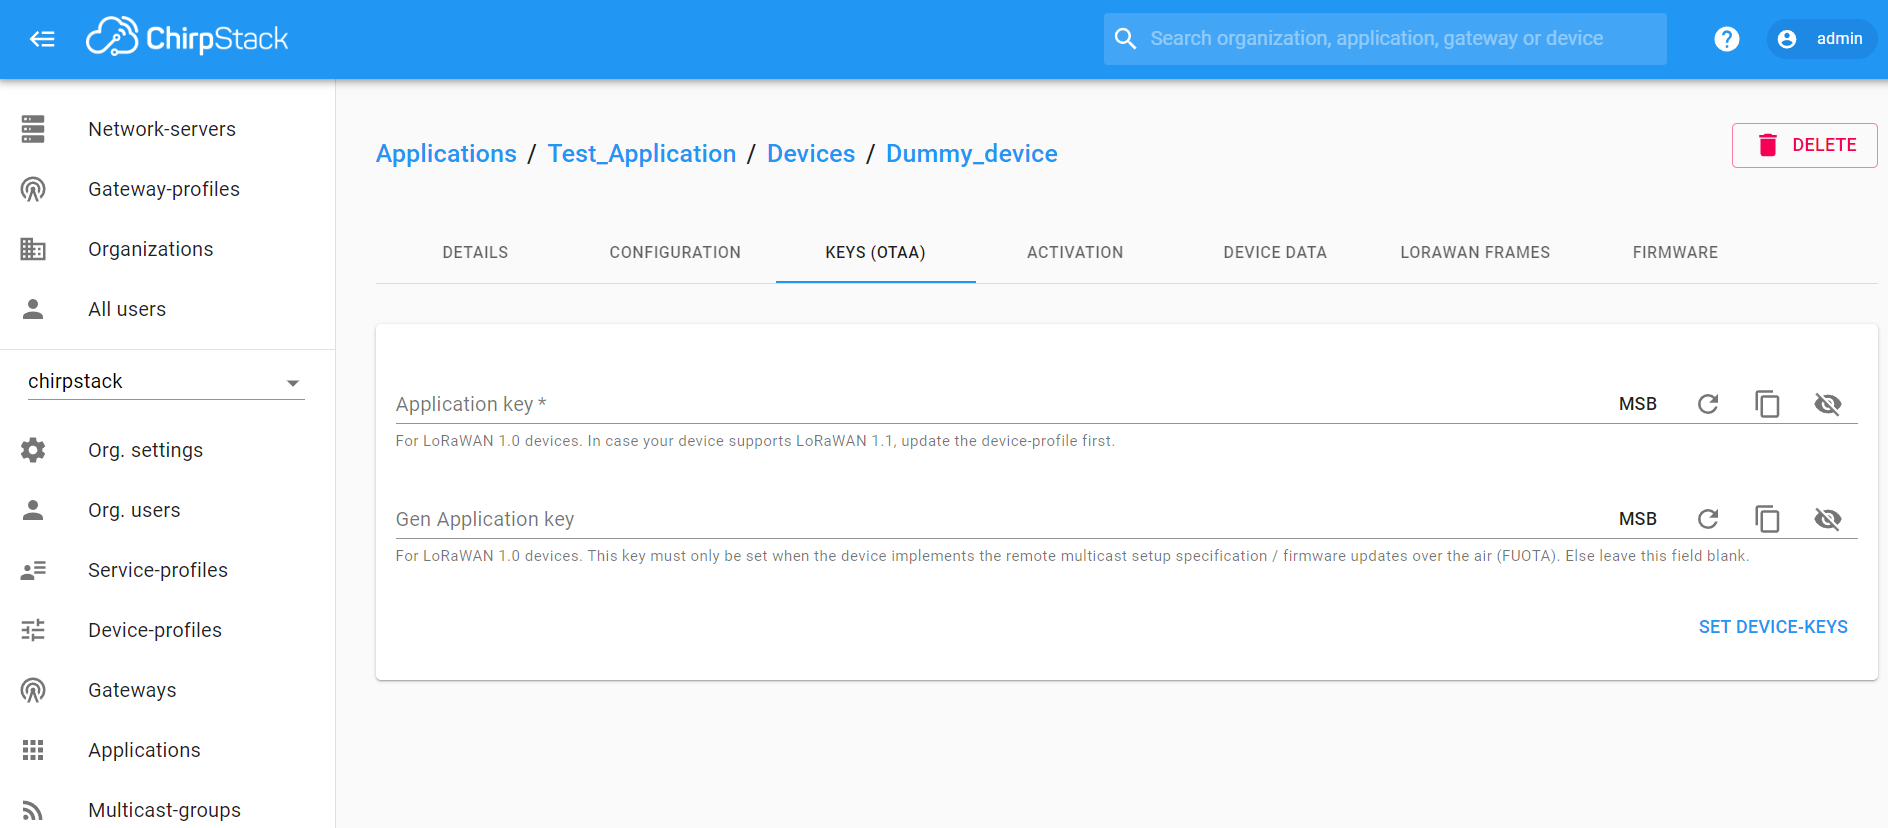
\includegraphics[width=\textwidth]{illustration/Chirpstack_new_device_2.png}}
  \caption{Keys (\gls{otaa}) information form for adding a new device to the application}
  \label{fig:chirpstack_new_device_2}
\end{figure}

Device can only be added once to the Chirpstack server and if it is tried to add another time to either the same application it already exists on or to a new one the process fails with an error message.

%\cite{chirpstack:devices}

\clearpage %force the next chapter to start on a new page. Keep that as the last line of your chapter!
